\chapter{Overview of the Previous Work}

\section{The history of Self Organizing Map (SOM)}
Self-Organizing Map (SOM), also know as Kohonen map, is a topological preserving map that can map a higher dimensional space to a lower dimensional space. Along this process, information will be compressed; while, the key parameters in terms of "topological and metric relationships"\cite{Kohonen1998} will be retained. 
\\
There are two steps involved in forming a self-organizing map from a raw input data-set\cite{hebbian2007}, respectively to be 1) \textbf{competition} and 2) \textbf{cooperation}. When a set of data is feed into the system sequentially with random shuffle, for each input data point, \textbf{competition} will take place first and, based on a pre-defined cost function, one of the neurons on the output layer with the minimal cost will be selected as a winner; Following the competition, the  \textbf{cooperation} will then take place. Based on a neighbourhood function, the winner together with it's neighbour neurons will proceed the learning; while, the neurons outside of the winner's neighbour zone will gain no learning. The purpose of the cooperation step is to increase the like-hood that if a similar input pattern present again, the same group of neurons will become the winner with a higher possibility. Iterate with this strategy on the input data-set over a suitable period, without supervising (providing error to the system), the output layer will simultaneously form a map that contains the similar topological structure as the input data. 

\section{Solving the task scheduling problem with SOM }
\subsection{Task scheduling with K output neurons}
In 2006, based on the SOM approach, Anmin and Simon proposed a new method to solve the multi-robot system problems in a multi-agent architecture\cite{zhu2006k}. In this research, robots are scheduled to approach the targets by competition and cooperation. 
\\
The robots and targets are assumed to be randomly initialized in a bounded area. Conventional method are limited with the restriction that all the targets are static. However, in this algorithm proposed by Anmin, the path planning and robots’ movements start synchronously. The left panel in Figure \ref{fig-2} shows the model of this architecture: there are 2 neurons on the input layer and K neurons on the output layer that are representing the coordinate locations of the target and the coordinate locations of the K robots, respectively. The K connecting weight vectors, $\{w_jx , w_jy\}$, where j = 1, 2, …, K, are computed from the Euclid distance between the input task and the location of each of the robots. In each epoch, the robot with the lowest distance is selected as the winner and the weight vectors within the winner’s neighbourhood zone will be updated to approaching the input target. All the targets will be input to the model in a random sequence in each iteration.

\begin{figure}[h]
  \centering
  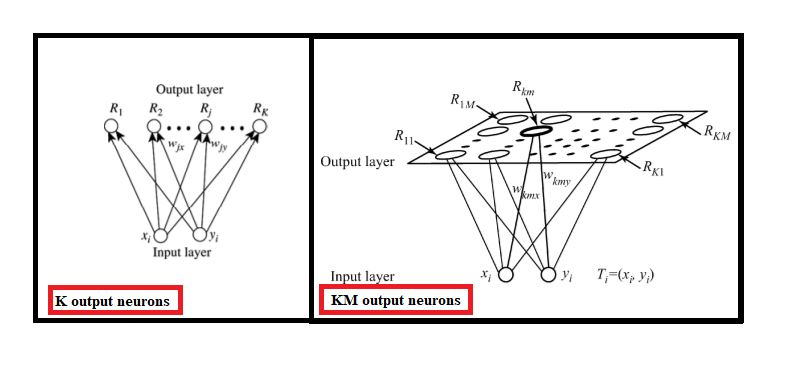
\includegraphics[width=15cm]{Pictures/SimonAmin2Methods.JPG}
  \caption{The illustration of two SOM configuration\cite{zhu2006neural,zhu2006k}.}
  
  \Description{The figure on the left has $K$ neurons on the output layer\cite{zhu2006k}; while, the figure on the right has $KM$ neurons on the output layer\cite{zhu2006neural}}
  \label{fig-2}
\end{figure}

Another interesting idea in this paper is the path planning for multi-robot systems. Several depots randomly distribute in the area. The task for robots is to get the goods from depots and reach the destination in the end. Thus, K M nodes are used in this task. Each robot has a group of M neuron to do the planning of K paths for robots. Here, each neurons used a term P to control the workload for each robot. The distance computation is multiplied by the term P, which is regards as:

\begin{equation}
    P = \frac{{L + V}}{{1 + V}}
\end{equation}

Where, L represent the path of the robot and V is the average path length. 
\subsection{Task Scheduling with KM output neurons}
As illustrating on the right panel of Figure \ref{fig-2}, Anmin had also proposed a different method to solve this problem. In the second paper\cite{zhu2006neural}, the K M neurons are used in the second layer of self-organizing map to do the path planning for dynamic task. For path planning problems, the M neurons are assigned to a group for K robots. Also, the P control is also used to balance the workload for K robots as the previous paper. By doing this, the dynamic trajectories can be recorded with workload balance.  In this task, the targets move a step in a random direction in each iteration. And the robot can still get to the target successfully. Although the path is not a near-optimal solution for the task, the task can be completed in computational time. 